% !TeX program = lualatex
% !TeX root = luaking.tex
% !TeX encoding = UTF-8
% !TeX spellcheck = cs_CZ
%---------------------------------------------------------------------------------------------------
% file magn1ch03.tex
\graphicspath{{../src/TEO/img/}}
%===================== Kapitola: Elektromagnetické pole ============================================
\setchaptertoc
\chapter{Elektromagnetické pole}\label{ES:kap_elmagp}

  
  Cílem kapitoly je připravit teoretickou půdu především pro 4. kapitolu, ve které bude podrobně 
  řešen magnetický a elektrický skinefekt a s ním související praktické problémy, týkající se 
  zvýšených ztrát v železe i zvýšených ztrát ve vinutí transformátorů a tlumivek. 
  
  V této kapitole bude elektromagnetické pole analyzováno pouze v prostředí, které se vyznačuje 
  následujícími vlastnostmi:
  \begin{itemize}[noitemsep]
    \item Prostředí je lineární: \(D = \varepsilon E\), \(B = \mu H\), \(E=\varrho J\).
    \item Prostředí je \textbf{homogenní}: parametry \(\varepsilon\), \(\mu\), \(\varrho\) jsou 
          stejně velké ve všech bodech prostoru, tzn. jsou nezávislé na souřadnicích \(x\), (y), 
          \(z\).
    \item Prostředí je \textbf{izotropní}: parametry \(\varepsilon\), \(\mu\), \(\varrho\) jsou 
          stejně velké ve všech směrech prostoru\footnote{Příkladem neizotropního prostředí je 
          transformátorový ocelový plech válcovaný zastudena. Ten má ve směru válcování větší 
          permeabilitu než ve směru příčném. V takovém případě je nutno hovořit o dvojrozměrném 
          tenzoru permeability - tenzor má tvar matice o rozměru \(2\times2\).}.
    \item Vyšetřovaný prostor \emph{neobsahuje} vnitřní zdroje elektromagnetické energie, tzn. 
          elektromagnetická vlna vniká do sledovaného prostoru \emph{zvenčí} a poté se v něm pouze 
          šíří.
    \item V prostoru se nevyskytují volné náboje\footnote{V elektricky vodivých kovech se vyskytují 
          volné elektrony. Jejich náboj je však vykompenzován kladnými ionty krystalové mřížky. 
          Je-li vlnová délka elektromagnetické vlny podstatně delší než vzdálenost mezi dvěma 
          sousedními atomy v mřížce (a tato nerovnost je v běžné technické praxi splněna vždy, 
          přestává platit až v rentgenové oblasti), pak lze vnitřek krystalu považovat za 
          elektricky neutrální, neboť ve střední hodnotě se náboje volných elektronů a iontů 
          dokonale kompenzují (i když teče kovem vodivý proud pohybujících se elektronů).}, tzn. 
          objemová hustota náboje\footnote{Objemová hustota náboje je označena \(\varrho_Q\), aby 
          byla odlišena od měrného odporu \(\varrho\).} je nulová, \(\varrho_Q = 0\).
  \end{itemize}
  
  Za těchto předpokladů bude v následujících kapitolách ukázáno, že všechny veličiny 
  elektromagnetického pole \(\vec{E}\), \(\vec{D}\), \(\vec{H}\), \(\vec{B}\) vyhovují známé vlnové 
  rovnici\footnote{V Maxwellově době byla tato rovnice běžně známa v mechanice (kmity) a v 
  termodynamice (Fourierův zákon šíření tepla).}:
  \begin{equation}\label{ES:eq_elmagp01}
    \Delta\vec{X}(x,y,z,t) - 
    \frac{\mu}{\varrho}\der{\vec{X}(x,y,z,t)}{t} - 
    \mu\varepsilon\dder{\vec{X}(x,y,z,t)}{t} = 0
  \end{equation}
  kde \(\Delta = \nabla^2\) je \emph{Laplaceův operátor}, \(\vec{X}\) je libovolná ze čtyř 
  jmenovaných veličin pole.
  
  \section{Vlnové rovnice elektromagnetického pole}
    Z matematického hlediska je nutno mít na zřeteli, že Maxwellovy rovnice tvoří soustavu 
    \emph{čtyř} parciálních diferenciálních rovnic o \emph{čtyřech} \emph{neznámých 
    prostoročasových vektorových funkcích} \(\vec{E}\), \(\vec{D}\), \(\vec{H}\), \(\vec{B}\) 
    (zkráceně o čtyřech veličinách \(\vec{E}\), \(\vec{D}\), \(\vec{H}\), 
    \(\vec{B}\))\footnote{Každý vektor příslušné veličiny \(\vec{E}\), \(\vec{D}\), \(\vec{H}\), 
    \(\vec{B}\) je funkcí prostorových souřadnic \(x\), \(y\), \(z\) a času \(T\). V tomto smyslu 
    má pak označení veličina a funkce (oné veličiny) stejný význam.}. S ohledem na zmíněnou 
    \emph{linearitu}, \emph{homogenitu} a \emph{izotropii} prostředí je možno psát materiálové 
    rovnice prostředí v následujícím vektorovém tvaru:
    \begin{equation}\label{ES:eq_elmagp02}
      \vec{D} = \varepsilon\vec{E}, \quad \vec{B} = \mu\vec{H}, \quad \vec{E} = 
      \frac{\vec{J}}{\varrho}
    \end{equation}
    Pomocí nich lze \emph{postupně} eliminovat ze soustavy čtyř Maxwellových rovnic jednotlivé 
    funkce, až vznikne \emph{jedna diferenciální rovnice o jedné neznámé funkci}, tj. 
    \textbf{vlnová rovnice} (\ref{ES:eq_elmagp01}). Například můžeme eliminovat funkce \(\vec{D}\), 
    \(\vec{B}\) tak, že v soustavě se budou vyskytovat pouze zbývající dvě veličiny \(\vec{E}\), 
    \(\vec{H}\):
    \begin{subequations}
      \begin{align}
        \rot{H}   &= \vec{J} + \der{\vec{D}}{t} 
                     \qquad \Rightarrow \boxed{\rot{H} 
                       = \frac{\vec{E}}{\varrho} + 
                         \varepsilon\der{\vec{E}}{t}}\, ,    \label{ES:eq_elmagp03a} \\
        \rot{E}   &= - \der{\vec{B}}{t}
                     \qquad\quad\, \Rightarrow \boxed{\rot{E} 
                       = -\mu\der{\vec{H}}{t}}\, ,           \label{ES:eq_elmagp03b} \\
        \diver{B} &= 0 \qquad\qquad\quad \Rightarrow \boxed{\diver{H} 
                       = 0}\, ,                              \label{ES:eq_elmagp03c} \\
        \diver{D} &= \varrho_Q = 0 \quad\quad\,\,\, \Rightarrow \boxed{\diver{E}
                       = 0}\, .                              \label{ES:eq_elmagp03d}
      \end{align}
    \end{subequations}
    Na obě strany rovnice (\ref{ES:eq_elmagp03b}) lze aplikovat operaci \textbf{rot} a následně 
    zaměnit vzniklou \(\rot{H}\) rovnicí (\ref{ES:eq_elmagp03a}). Poté lze využít známé operátorové 
    identity vektorového počtu \(\text{rot}\,\text{rot} = \text{grad}\,\text{div} -\Delta\). 
    Naznačená posloupnost kroků bude mít následující konkrétní podobu:
    \begin{align}
     \text{rot}\,\rot{E} &= -\mu\der{}{t}\rot{H} 
                          = -\mu\der{}{t}
                             \left(
                               \frac{\vec{E}}{\varrho} +
                               \varepsilon\der{\vec{E}}{t}
                              \right)                            \nonumber  \\
                         &= - \frac{\mu}{\varrho}\der{\vec{E}}{t} - 
                              \mu\varepsilon\dder{\vec{E}}{t} 
                          = \text{grad}\,\diver{E} - \Delta\vec{E}  \label{ES:eq_elmagp04}
    \end{align}
    S ohledem na (\ref{ES:eq_elmagp03d}) musí platit \(\text{grad}\,\diver{E} = 0\). Tak získáme 
    konečný tvar vlnové rovnice pro vektor \(\vec{E}\):
    \begin{equation}\label{ES:eq_elmagp05}
      \Delta\vec{E} - \frac{\mu}{\varrho}\der{\vec{E}}{t} - \mu\varepsilon\dder{\vec{E}}{t} = 0
    \end{equation}
    Aplikujeme-li rotaci na rovnici (\ref{ES:eq_elmagp03a}), lze stejným postupem získat identickou 
    vlnovou rovnici pro vektor \(\vec{H}\). Z vlnových rovnic pro obě intenzity \(\vec{E}\), 
    \(\vec{H}\) lze pomocí vztahů (\ref{ES:eq_elmagp02}) snadno určit zbývající vlnové rovnice pro 
    obě indukce \(\vec{D}\), \(\vec{B}\). Všechny čtyři rovnice budou formálně identické. Zbývající 
    tři rovnice mají tedy tvar
    \begin{subequations}
      \begin{align}
        \Delta\vec{H} - \frac{\mu}{\varrho}\der{\vec{H}}{t} 
          - \mu\varepsilon\dder{\vec{H}}{t} &= 0   \label{ES:eq_elmagp06a}          \\
        \Delta\vec{D} - \frac{\mu}{\varrho}\der{\vec{D}}{t} 
          - \mu\varepsilon\dder{\vec{D}}{t} &= 0   \label{ES:eq_elmagp06b}          \\
        \Delta\vec{B} - \frac{\mu}{\varrho}\der{\vec{B}}{t} 
          - \mu\varepsilon\dder{\vec{B}}{t} &= 0   \label{ES:eq_elmagp06c}
      \end{align}
    \end{subequations}

    
    Jedná se o lineární parciální diferenciální rovnice druhého stupně pro jednotlivé funkce 
    (veličiny). Převrácená hodnota \(\frac{1}{\mu\varepsilon}\) má význam \emph{čtverce fázové 
    rychlosti}, s jakou se pole šíří prostředím. Konstanta \(\frac{\mu}{\varepsilon}\) o rozměru 
    \([s/m^2]\) má význam \emph{měrného tlumení}. Pro izolanty je tlumení zřejmě nulové a vlna se 
    šíří prostředím bez útlumu. Z fyzikálního rozměru lze poznat, že tlumicí konstantu je možno 
    chápat i jako \emph{měrnou časovou konstantu}. Skutečná časová konstanta \(\tau\) určitého 
    objemu \(V=l^3\) o lineárních rozměrech \(l\) je pak totiž úměrná čtverci \(l^2\) těchto 
    rozměrů. To je obecně známá vlastnost z mnoha oblastí fyziky (např. šíření tepla, mechanika ve 
    3D prostoru, magnetické jevy v plazmatu atd.).
  
  \section{Řešení vlnových rovnic}
    Parciální diferenciální rovnice (\ref{ES:eq_elmagp05}) až (\ref{ES:eq_elmagp06c}) jsou velmi 
    těžko řešitelné analyticky v uzavřeném tvaru. Výjimkou je případ, kdy se jedná o harmonické 
    signály v ustáleném stavu. V tom případě mají totiž všechny vektory \(\vec{E}\), \(\vec{D}\), 
    \(\vec{H}\), \(\vec{B}\) harmonické časové průběhy o stejném kmitočtu, ale o různých 
    amplitudách a různých fázových posuvech, neboť amplitudy\footnote{V celé 3. kapitole budeme 
    pracovat s amplitudami, nikoli s efektivními hodnotami.} i fázové posuvy jsou funkcemi 
    prostorových souřadnic. Např. vektor \(\vec{E}\) lze zapsat ve složkovém tvaru:
    \begin{align}
     \vec{E}(x,y,z,t) &= E_x(x,y,z,t)\cos(\omega t - \varphi_x(x,y,z,t))  \nonumber   \\
                      &+ E_y(x,y,z,t)\cos(\omega t - \varphi_y(x,y,z,t))  \nonumber   \\
                      &+ E_z(x,y,z,t)\cos(\omega t - \varphi_z(x,y,z,t))  \label{ES:eq_elmagp07} 
    \end{align}
    Záporné znaménko u fázových posuvů \(\varphi\) vyjadřuje skutečnost, že vlna se fázově zpožďuje 
    při postupu ve směru kladných os \(x\), \(y\), \(z\). V následujících kapitolách budeme řešit 
    rovinnou a lineárně polarizovanou elektromagnetickou vlnu, šířící se v různých fyzikálních 
    prostředích, majících rozdílné vlastnosti \(\mu\), \(\varepsilon\), \(\varrho\).
    
    \subsection{Rovinná vlna v obecném prostředí}
    
      \begin{figure}[ht!]
        \centering
        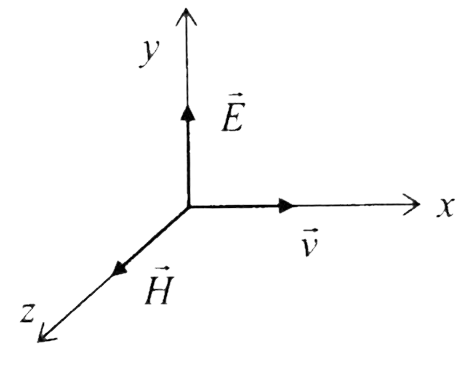
\includegraphics[width=0.7\linewidth]{patocka_elmgp01.png}
        \caption{Čelo rovinné vlny je orientováno rovnoběžně s rovinou \(y-z\) a šíří se ve směru 
                 kladné osy \(x\) fázovou rychlostí \(v\).\cite[s.~70]{Patocka4}}
        \label{ES:fig_elmgp01}
      \end{figure}
      Tato kapitola řeší nejobecnější případ, ve kterém nelze zanedbat ani jednu vlastnost \(\mu\), 
      \(\varepsilon\), \(\varrho\) prostředí, v němž se vlna šíří. V kapitolách navazujících pak 
      budou řešeny zvláštní případy\footnote{Bude se jednat především o izolanty, polovodiče a 
      dobré vodiče (tj. všechny kovy).} plynoucí z tohoto obecného řešení. 
  
      Pro zjednodušení výpočtů, avšak bez újmy na obecnosti, budeme orientovat čelo rovinné vlny 
      paralelně se souřadnou rovinou \(y-z\). Podle obr. \ref{ES:fig_elmgp01} se čelo vlny šíří 
      rychlostí \(v\) ve směru kladné osy \(x\).
      
      Vektor \(\vec{E}\) je ztotožněn s osou \(y\), tedy platí
      \begin{equation}\label{ES:eq_elmagp08}
         E_x = 0, \qquad E_z = 0.
      \end{equation}
      Pak existuje pouze jediná složka \(E_y\), proto se Laplacián \(\Delta\vec{E}\) zjednoduší do 
      tvaru
      
      \begin{align*}                  % \label{ES:eq_elmagp09}
        \Delta\vec{E} &= \ppder{E(x,y,z,t)}{x} + 
                         \ppder{E(x,y,z,t)}{y} + \ppder{E(x,y,z,t)}{z}      \\
                      &= \ppder{E_y(x,y,z,t)}{x} + 
                         \ppder{E_y(x,y,z,t)}{y} + \ppder{E_y(x,y,z,t)}{z}
      \end{align*}
      Vlna je v nekonečné rovině \(y-z\) \emph{homogenní}, proto musí pro její jedinou složku 
      \(E_y\) platit
      \begin{equation}\label{ES:eq_elmagp10}
        \pder{E_y}{y} = 0, \qquad \pder{E_y}{z} = 0.
      \end{equation}
      To vede k dalšímu zjednodušení Laplaciánu \(\Delta\vec{E}\) do podoby
      \begin{equation}\label{ES:eq_elmagp11}
        \Delta\vec{E} = \ppder{E_y(x,y,z,t)}{x} + 0 + 0 = \ppder{E_y(x,t)}{x}
      \end{equation}
      Vlnová rovnice (\ref{ES:eq_elmagp05}) pak nabude tvaru parciální diferenciální rovnice dvou 
      proměnných \(x\), \(t\)
      \begin{equation}\label{ES:eq_elmagp12}
        \ppder{E_y(x,t)}{x} + 
        \frac{\mu}{\varrho}\der{E_y(x,t)}{t} - 
        \mu\varepsilon\dder{E_y(x,t)}{t} = 0
      \end{equation}
      V uzavřeném tvaru lze tuto rovnici řešit pouze pro \emph{harmonické} veličiny metodou 
      \emph{separace proměnných}. Je-li tedy veličina \(E_y(x,t)\) \emph{reálnou} funkcí 
      \emph{harmonicky} závislou na čase \(t\) a současně i na souřadnici \(x\) podle rovnice 
      (\ref{ES:eq_elmagp07}), formálně je možno této reálné veličině přiřadit \emph{komplexní}
      vektor, neboli \textbf{fázor} \(\hat{E}_y(x,t)\) mající tvar
      \begin{equation}\label{ES:eq_elmagp13}
        \hat{E}_y(x,t) = Ee^{j(\omega t - kx)} = Ee^{-jkx}e^{\omega t},
      \end{equation}
      kde \(E\) je \emph{amplituda} vlny, \(k\) je \emph{činitel šíření}. Záporné znaménko u členu 
      \(-kx\) vyjadřuje skutečnost, že vlna se při postupu ve směru \emph{kladné} osy \(x\) fázově 
      zpožďuje (nelze porušit kauzalitu času). Zavedením komplexního fázoru se podařilo obě 
      proměnné \(x\), \(t\) separovat, protože fázor získal tvar \(\hat{E}(x,t) = E\times f_1(x) 
      \times f_2(t)\) součinu dvou funkcí jednotlivých proměnných. Komplexní funkce 
      (\ref{ES:eq_elmagp13}) je současně řešením parciální diferenciální rovnice 
      (\ref{ES:eq_elmagp12}), ovšem pokud se podaří najít neznámý parametr \(k\) takový, aby 
      rovnici vyhovoval. Určíme-li první a druhé parciální derivace, prozatím obecného 
      fázoru (\ref{ES:eq_elmagp13}), podle jednotlivých proměnných \(x\), \(t\) a dosadíme-li tyto 
      derivace do rovnice (\ref{ES:eq_elmagp12}), získáme vztah
      \begin{equation}\label{ES:eq_elmagp14}
        -k^2E -j\omega\frac{\mu}{\varrho}E +\mu\varepsilon\omega^2E^2 = 0.
      \end{equation}
      \subsubsection{Činitel šíření \(k\)}
        Po vydělení rovnice (\ref{ES:eq_elmagp14}) amplitudou \(E\) získáme jednoduchou 
        algebraickou rovnici pro neznámý parametr \(k\). Řešením této kvadratické rovnice jsou dva 
        komplexní kořeny
        \begin{equation}\label{ES:eq_elmagp15}
          k_{1,2} = \pm\sqrt{\omega^2\mu\varepsilon - j\omega\frac{\mu}{\varrho}}
                  =\pm(\alpha-j\beta).
        \end{equation}
      \subsubsection{Fázová konstanta \(\alpha\), činitel tlumení \(\beta\), hloubka vniku 
                      \(\delta\)}
        Tyto parametry plynou po úpravě\footnote{Odmocninu z komplexního čísla lze snadno řešit v 
        polárním tvaru.} přímo z rovnice (\ref{ES:eq_elmagp15}). Výsledky mají tvar
        \begin{subequations}
          \begin{align}
            \alpha &= \omega\sqrt{
                              \frac{\mu\varepsilon}{2}
                                \left(
                                  \sqrt{1+\frac{1}{\omega^2\varrho^2\varepsilon^2}} +1 
                                \right)}                
                      \qquad\qquad [\si{\radian/\meter}]  \label{ES:eq_elmagp16a}  \\
            \beta  &= \frac{1}{\delta} 
                    = \omega\sqrt{
                              \frac{\mu\varepsilon}{2}
                                \left(
                                  \sqrt{1+\frac{1}{\omega^2\varrho^2\varepsilon^2}} -1
                                \right)}               
                      \qquad [\si{1/\meter}]               \label{ES:eq_elmagp16b}
          \end{align}
        \end{subequations}
        Hloubka vniku \(\delta\) je převrácenou hodnotou činitele tlumení \(\beta\) a má význam 
        vzdálenosti, na které klesne amplituda dopředně vlny na hodnotu \(1/e\) po vniknutí do 
        materiálu. Je vidět, že \(\beta\) i \(\delta\) jsou určitě čísla \emph{kladná}, dopředná 
        vlna \(E_+\) tedy opravdu exponenciálně slábne při průchodu prostředím s parametry \(\mu\), 
        \(\varepsilon\), \(\varrho\). Kladný činitel šíření \(k_1=+(\alpha-j\beta)\) odpovídá 
        \textbf{dopředné vln} \emph{postupující ve směru} \(+x\), záporný činitel šíření 
        \(k_2=-(\alpha-j\beta)\) odpovídá \textbf{zpětné vlně} \emph{odražené}, postupující ve 
        směru \(-x\). Výsledné řešení může být v obecném případě superpozicí obou vln. V úvahu 
        připadají následující obecné možnosti. Dosadíme-li (\ref{ES:eq_elmagp15}) do 
        (\ref{ES:eq_elmagp13}), lze tyto možnosti rozepsat takto:
        \begin{subequations}
          \begin{align}
            \shortintertext{vlna dopředná:}
            \hat{E}_y(x,t) 
              &= E_+e^{j(\omega t - kx)}                               \nonumber \\
              &= E_+e^{-\beta x}e^{j(\omega t-\alpha x)}                 
               = E_+e^{-\frac{x}{\delta}}e^{j(\omega t-\alpha x)}      \label{ES:eq_elmagp17a} \\
            \shortintertext{vlna zpětná:}
            \hat{E}_y(x,t) 
              &= E_-e^{j(\omega t + kx)}                               \nonumber \\
              &= E_-e^{+\beta x}e^{j(\omega t+\alpha x)}                 
               = E_-e^{+\frac{x}{\delta}}e^{j(\omega t+\alpha x)}      \label{ES:eq_elmagp17b} \\
            \shortintertext{vlna dopředná \(\pm\) zpětná:}
            \hat{E}_y(x,t) 
              &= E_+e^{j(\omega t - kx)} \pm E_-e^{j(\omega t +kx)}    \nonumber \\
              &= E_+e^{-\beta x}e^{j(\omega t-\alpha x)} 
                 \pm E_-e^{+\beta x}e^{j(\omega t+\alpha x)}           \nonumber \\ 
              &= E_+e^{-\frac{x}{\delta}}e^{j(\omega t-\alpha x)}
                 \pm E_-e^{+\frac{x}{\delta}}e^{j(\omega t+\alpha x)}  \label{ES:eq_elmagp17c} 
          \end{align}
          V obecném případě nemusí mít amplitudy \(E_+\) a \(E_-\) stejnou velikost. Tak je tomu 
          např. při odrazu a lomu vlny na rozhraní dvou různých prostředí. Při analýze 
          \emph{skinefektu} uvnitř tenkého plechu lze díky osové symetrii ve směru tloušťky plechu, 
          tj. osy \(x\), položit \(E_+=E_-= \frac{E(0)}{2}\), kde \(E(0)\) je středová hodnota pro 
          \(x = 0\). Pak je možno rovnici (\ref{ES:eq_elmagp17c} ) upravit buď do tvaru
          \begin{align}
            \shortintertext{vlna „dopředná“ + „zpětná“:} 
            \hat{E}_y(x,t) &= E_+e^{j(\omega t - kx)} + E_-e^{j(\omega t + kx)}    \nonumber \\
                           &= \frac{E(0)}{2}e^{j(\omega t - kx)} + 
                              \frac{E(0)}{2}e^{j(\omega t + kx)}                   \nonumber \\
                           &= E(0)\cosh(jkx)e^{j\omega t}         \label{ES:eq_elmagp18a}    \\
            \shortintertext{nebo do tvaru}
            \shortintertext{vlna „dopředná“ - „zpětná“:} 
            \hat{E}_y(x,t) &= E_+e^{j(\omega t - kx)} - E_-e^{j(\omega t + kx)}    \nonumber \\
                           &= \frac{E(0)}{2}e^{j(\omega t - kx)} + 
                              \frac{E(0)}{2}e^{j(\omega t + kx)}                   \nonumber \\
                           &= E(0)\cosh(jkx)e^{j\omega t}         \label{ES:eq_elmagp18b}
          \end{align}
        \end{subequations}
        V případě \emph{skinefektu} nelze fyzikálně interpretovat součet obou dílčích řešení jako 
        součet vlny \uv{dopředné} a \uv{zpětné}, nicméně výsledná řešení (\ref{ES:eq_elmagp17a} 
        -\ref{ES:eq_elmagp18b}) mají uvedený tvar, jsou skutečně správná a odpovídající realitě.

      \subsubsection{Fázová rychlost}
        Fázovou rychlost, s jakou se vlna šíří, lze určit jako rychlost \emph{geometrického místa 
        konstantní fáze vlny}. Toto místo plyne pro \emph{dopřednou} vlnu z (\ref{ES:eq_elmagp17a}) 
        a je určeno podmínkou
        \begin{equation}\label{ES:eq_elmagp19}
          \omega t-\alpha x = \text{konst.}\qquad\Rightarrow
                          x = \frac{\omega t - \text{konst.}}{\alpha}.
        \end{equation}
        Odtud lze určit fázovou rychlost jako derivaci dráhy \(x\) podle času \(t\):
        \begin{align}\label{ES:eq_elmagp20}
          v  = \der{x}{t} = \frac{\omega}{\alpha}
            &= \frac{1}{\sqrt{\mu\varepsilon}}
               \sqrt{\dfrac{2}{1+\sqrt{1+\dfrac{1}{\omega^2\varrho^2\varepsilon^2}}}} \nonumber \\
            &= v_0\sqrt{\dfrac{2}{1+\sqrt{1+\dfrac{1}{\omega^2\varrho^2\varepsilon^2}}}},
        \end{align}
        kde \(v_0\) je rychlost netlumené vlny v bezeztrátovém nevodivém prostředí při \(\varrho 
        \rightarrow\infty\). Vidíme, že ve ztrátovém prostředí (i pouze mírně vodivém, zvláště 
        pak v kovech) bude vždy platit \(v < v_0\). Do vnitřního prostoru supravodičů 
        elektromagnetické vlny vůbec vniknout nemohou, protože pro \(\varrho = 0\) vychází rychlost 
        vnikající vlny \(v = 0\). To je v plném souladu se závěry z příkladu na obrázku 
        \ref{teo:fig042} na konci kapitoly \ref{teo:IchapIIsecI}.
        
        Zajímavá je rovněž závislost rychlosti na kmitočtu. Pro \(\omega = 0\) je \(v = 0\), tj. 
        statické pole se nešíří v prostoru. Pro \(\omega\rightarrow\infty\) platí \(v = v_0\), 
        což je v souladu s tím, že \(\gamma\)-záření se snadno šíří i skrze kovy. Mezi vlnovou 
        délkou a fázovou rychlostí vlny platí známé vztahy
        \begin{equation}\label{ES:eq_elmagp21}
          \lambda = vT = \frac{v}{f} = 2\pi\frac{2}{\omega}
        \end{equation}

      \subsubsection{Vlnová impedance prostředí}
        Obecně má vektor \(\rot{E}\) tři složky
        \begin{align}
          (\text{rot}\,\vec{E})_x &=\left(\pder{E_z}{y}-\pder{E_y}{z}\right), \nonumber \\
          (\text{rot}\,\vec{E})_y &=\left(\pder{E_x}{z}-\pder{E_z}{x}\right), \nonumber \\
          (\text{rot}\,\vec{E})_z &=\left(\pder{E_y}{x}-\pder{E_x}{y}\right). \label{ES:eq_elmagp22}
        \end{align}
        Pro rovinnou vlnu platí zjednodušující podmínky (\ref{ES:eq_elmagp08}), plynoucí ze zvolené 
        orientace vektoru \(\vec{E}\), a navíc další podmínky (\ref{ES:eq_elmagp10}), plynoucí z 
        homogenity vlny. Všechny tyto podmínky vedou na značné zjednodušení složek rotace:
        \begin{equation}\label{ES:eq_elmagp23}
          (\text{rot}\,\vec{E})_x = 0, \quad
          (\text{rot}\,\vec{E})_y = 0, \quad
          (\text{rot}\,\vec{E})_z = \pder{E_y}{x}.
        \end{equation}
        Samotný vektor \(\vec{E}\) má \emph{jedinou} složku \(E_y\) ve směru osy \(y\). Je ale 
        vidět, že jeho rotace \(\rot{E}\) má naopak \emph{jedinou} složku ve směru osy \(z\). Proto 
        z druhé Maxwellovy rovnice
        \begin{equation}\label{ES:eq_elmagp24}
          (\rot{E} = -\der{\vec{B}}{t} = -\mu\der{\vec{H}}{t}
        \end{equation}
        ihned plyne, že vektor magnetického pole \(\vec{H}\) má také \emph{jedinou} složku, ale ve 
        směru osy \(z\). Tato složka \(H_z\) je tudíž \emph{kolmá} na složku \(E_y\). Druhá 
        Maxwellova rovnice totiž nabude tvaru
        \begin{equation}\label{ES:eq_elmagp25}
          (\text{rot}\,\vec{E})_z = - \der{B_z}{t} = -\mu\der{H_z}{t}.
        \end{equation}
        \begin{figure}[ht!]   
          \centering
          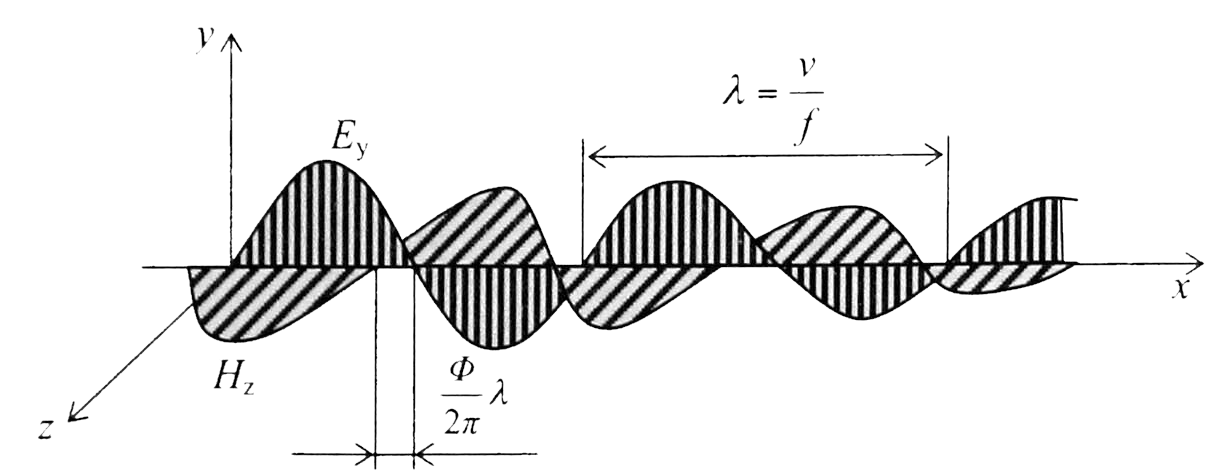
\includegraphics[width=0.95\linewidth]{patocka_elmgp02.png}
          \caption{Průběhy složek \(E_y\) a \(H_z\) v rovinné vlně, orientované paralelně s rovinou 
                   \(y-z\). Vlna se šíří obecným prostředím ve směru osy \(x\). Obě amplitudy se 
                   exponenciálně zmenšují. Magnetická složka je opožděna o úhel \(\Phi\) za 
                   elektrickou složkou \(E_y\). \cite[s.~74]{Patocka4}.}
          \label{ES:fig_elmgp02}
        \end{figure}
        Pravé strany rovnic (\ref{ES:eq_elmagp24}) a (\ref{ES:eq_elmagp25}) se musí sobě rovnat. 
        Tak získá druhá Maxwellova rovnice \emph{rovinné vlny} jednoduchý tvar
        \begin{equation}\label{ES:eq_elmagp26}
          \boxed{\pder{E_y}{x} = - \mu\der{H_z}{t}}.
        \end{equation}
        Nyní uvažujme složku \(E_y\) v komplexním tvaru \(\hat{E}_y(x,t)=Ee^{j(\omega t - kx)}\)  
        podle rovnice (\ref{ES:eq_elmagp13}). Podobně zavedeme i komplexní fázor \(\hat{H}_z\) pro 
        složku \(H_z\):
        \begin{equation}\label{ES:eq_elmagp27}
          \hat{H}_z(x,t)=H e^{j(\omega t - kx)}.
        \end{equation}
        Ve shodě s rovnicí (\ref{ES:eq_elmagp26}) derivujme nyní rovnici (\ref{ES:eq_elmagp13}) 
        podle souřadnice \(x\) a rovnici (\ref{ES:eq_elmagp27}) podle času \(t\). Dosadíme-li obě 
        derivace do druhé Maxwellovy rovnice (\ref{ES:eq_elmagp26}), získáme jednoduchý vztah mezi 
        \emph{amplitudami} \(E\), \(H\) obou složek pole
        \begin{equation}\label{ES:eq_elmagp28}
          E = \frac{\omega\mu}{k}H.
        \end{equation}
        Poměrem amplitud \(E\) a \(H\) těchto složek pole je definována \textbf{vlnová impedance} 
        prostředí:
        \begin{align} \label{ES:eq_elmagp29}
          Z  = \frac{E}{H} = \frac{\omega\mu}{k}
            &= \sqrt{\dfrac{\mu}{\varepsilon}}
               \frac{1}{\sqrt{1-j\frac{1}{\omega\varrho\varepsilon}}}                 \nonumber \\
            &= \frac{1}{\sqrt{1+\frac{1}{\omega^2\varrho^2\varepsilon^2}}}e^{j\Phi}
             = \abs{Z}e^{j\Phi},
        \end{align}

        \begin{align}\label{ES:eq_elmagp32}
          \Phi &= -\arctan\frac{-\beta}{\alpha} = \arctan\frac{\beta}{\alpha}         \nonumber \\
               &=  \arctan\left[
                            \omega\varrho\varepsilon
                              \left(\sqrt{1+
                                 \frac{1}{\omega^2\varrho^2\varepsilon^2}}-1
                              \right)
                          \right].
        \end{align}
        Úhlem \(\Phi\) je definován fázový posuv mezi oběma vektory (v časové oblasti, tedy i v 
        prostoru ve směru osy \(x\)). Je vidět, že v obecném vodivém ztrátovém prostředí je vždy 
        \(\Phi>0\), složka \(H_z\) je tedy vždy opožděna za složkou \(E_y\) podle obr. 
        \ref{ES:fig_elmgp02}.
        
      \subsubsection{Elektromagnetické vnění je příčné}
        Tento fakt plyne názorně přímo z rolvnice (\ref{ES:eq_elmagp26}), z obr. 
        \ref{ES:fig_elmgp01} a z obr. \ref{ES:fig_elmgp02}. Méně zřetelně, zato však mnohem 
        obecněji, plyne přímo z modifikovaných Maxwellových rovnic (\ref{ES:eq_elmagp03c}) a 
        (\ref{ES:eq_elmagp03d}). Rozepíšeme-li totiž divergenci pro vektory \(\vec{E}\), 
        \(\vec{H}\), získají obě rovnice tvar
        \begin{subequations}
          \begin{align}\label{ES:eq_elmagp30}
            \diver{E} &= \pder{E_x}{x} + \pder{E_y}{y} + \pder{E_z}{z} = 0   \nonumber \\
            \diver{H} &= \pder{H_x}{x} + \pder{H_y}{y} + \pder{H_z}{z} = 0
          \end{align}
        \end{subequations}
        Předpokládejme nejdříve, že \emph{podélné} složky \(E_x\), \(H_x\) ve směru šířeni \(x\) 
        existují. Pokud ale existují, musí mít tvar vlny, tj. musí se periodicky měnit v závislosti 
        na souřadnici \(x\). Pak ale jejich derivace \(\pder{}{x}\) \emph{nemohou být nulové}. To 
        je však v rozporu s rovnicemi (\ref{ES:eq_elmagp30}), tedy i v rozporu s původním 
        předpokladem. Z rozporu plyne, že podélné složky \(E_x\), \(H_x\) ve směru šíření \(x\) 
        nemohou existovat. Naopak \emph{příčné} složky \(E_y\), \(E_z\), \(H_y\), \(H_z\), kolmé na 
        směr \(x\), nulové být nemusí s ohledem na homogenitu rovinné vlny v rovině \(y-z\). Z 
        \emph{homogenity} totiž plyne, že všechny derivace \(\pder{}{y}\), \(\pder{}{z}\) 
        budou \emph{určitě nulové}, i když nebudou nulové příslušné složky. Ze všech těchto 
        poznatků plyne, že tři vektory \(\vec{E}\), \(\vec{H}\), \(\vec{v}\) jsou v každém bodě 
        prostoru uspořádány do \textbf{ortogonálního} pravotočivého systému. 

      \subsubsection{Poyntingův vektor}
        Jeho okamžitá hodnota je definována vektorovým součinem
        \begin{equation}\label{ES:eq_elmagp31}
          \vec{\Gamma}(x,y,z,t)=\vec{E}(x,y,t)\times\vec{H}(x,y,z,t)
          \quad [\si{\W\per\square\m}; \si{\V\per\m}, 
                 \si{\A\per\m}],
        \end{equation}
        Odtud plyne, že i vektory \(\vec{E}\), \(\vec{H}\), \(\vec{\Gamma}\) tvoří v každém bodě 
        prostoru \emph{ortogonální pravotočivý systém}, neboť vektory \(\vec{\Gamma}\) a 
        \(\vec{v}\) mají vždy totožný směr i orientaci. Poyntingův\footnote{John Henry Poynting 
        (1852-1914), anglický fyzik, působil na univerzitě v Birminghamu. Zabýval se energií 
        elektromagnetického pole, měřením Newtonovy gravitační konstanty, sluneční radiací.} 
        vektor (\ref{ES:eq_elmagp31}) má význam plošné hustoty \emph{okamžitého} výkonu šířícího 
        se prostředím. Pro energetické úvahy je však podstatná plošná hustota \emph{středního} 
        neboli \emph{činného} výkonu šířícího se prostorem. Protože oba vektory \(\vec{E}\), 
        \(\vec{H}\) jsou harmonické a navíc v čase vůči sobě fázově posunuté o úhel \(\Phi\) daný 
        rovnicí (\ref{ES:eq_elmagp32}), platí pro činný neboli střední Poyntingův vektor 
        analogické vztahy jako pro činný výkon na lineární impedanci:
        \begin{align}\label{ES:eq_elmagp33}
          \Gamma_\text{č} \equiv \Gamma_\text{stř} 
            = \frac{1}{2}\Re\left[\hat{E}\hat{H}^*\right]
            &= \frac{1}{2}EH\cos\Phi 
            = \frac{1}{2}\frac{E^2}{\abs{Z}}\cos\Phi                  \nonumber \\
            &= \frac{1}{2}H^2\abs{Z}\cos\Phi.
        \end{align}
        V rovnicích figuruje koeficient \(\frac{1}{2}\), protože se jedná o \emph{amplitudy} 
        signálů. Přechod z amplitud na \emph{efektivní hodnoty} lze uskutečnit následujícím 
        způsobem:
        \begin{align}\label{ES:eq_elmagp34}
          \Gamma_\text{č} \equiv \Gamma_\text{stř} 
            = \frac{1}{2}EH\cos\Phi 
            &= \frac{1}{2}\frac{E}{\sqrt{2}}\frac{H}{\sqrt{2}}\cos\Phi   \nonumber \\
            &= \frac{1}{2}E_{ef}H_{ef}\cos\Phi.
        \end{align}
        Kromě využití v radiotechnice význam Poyntingova vektoru spočívá v možnosti výpočtu
        Jouleových ztrát v různých situacích: Například stačí zjistit hodnotu \(\Gamma_\text{č}\), 
        na povrchu vodiče a vynásobit ji plochou povrchu, tím určíme ztrátový Jouleův 
        výkon\footnote{Takto lze činný ztrátový výkon počítat pouze v případě, že do vnitřního 
        prostoru se energie nedostává ještě jiným způsobem - vyšetřovaný prostor nesmí obsahovat 
        vnitřní nezávislé zdroje.} ve vodiči \(P_{Cu} = R_{Cu}I_{ef}\). Poyntingův vektor na 
        povrchu vodiče totiž míří ze všech stran vždy dovnitř.
        
        Nyní je plně vyřešen problém šíření rovinné lineárně polarizované elektromagnetické vlny v 
        libovolném prostředí, které má obecné vlastnosti \(\varrho\), \(\mu\), \(\varepsilon\). Z 
        tohoto obecného řešení vyplynou v následujících kapitolách zvláštní případy pro různá 
        prostředí a různé materiály vyskytující se v technické praxi.

    \subsection{Rovinná vlna ve vakuu a v izolantech}
      Všechny následující výsledky jsou formulovány pouze pro vakuum, ale kvalitativně platí i 
      pro všechny ostatní izolanty, které se od vakua liší pouze jinými hodnotami \(\mu\), 
      \(\varepsilon\). Vakuum je dokonalý izolant s následujícími elektromagnetickými 
      vlastnostmi:
      \begin{equation}\label{ES:eq_elmagp35}
        \varrho\rightarrow\infty, \quad 
        \mu_0         =  \SI{4\pi e-7}{\henry\per\meter}, \quad
        \varepsilon_0 =  \SI{8.853e-12}{\F\per\meter}.
      \end{equation}
      Dosazení těchto hodnot do rovnic obecného řešení z předchozí kapitoly vede k následujícím 
      výsledkům.
 
      \subsubsection{Činitel šířeni \(k\)}
        S ohledem na \(\varrho\rightarrow\infty\) lze obecný výraz (\ref{ES:eq_elmagp15}) 
        pro činitel šíření k zjednodušit do podoby
        \begin{equation}\label{ES:eq_elmagp36}
          k_{1,2} = \pm\omega\sqrt{\mu\varepsilon_0} 
                  = \pm\frac{\omega}{c}
                  = \pm\alpha.
        \end{equation}
        Činitel šíření má pouze reálnou část, chybí imaginární útlumový člen, vakuum a izolanty 
        jsou tedy při přenosu elektromagnetické vlny \emph{bezeztrátové}.
           
      \subsubsection{Fázová konstanta \(\alpha\), činitel tlumení \(\beta\), hloubka 
                         vniku \(\delta\)}
        \begin{equation}\label{ES:eq_elmagp37}
          \alpha = \omega\sqrt{\mu_0\varepsilon_0} = \frac{\omega}{c}, \qquad 
          \beta  = 0,                                                  \qquad
           \delta = \rightarrow\infty.
        \end{equation}
        Činitel tlumení \(\beta\) je nulový, proto je hloubka vniku \(\delta\) nekonečná. Kladný 
        činitel šíření \(k_1 = +\alpha\), odpovídá dopředné vlně postupující ve směru \(+x\), 
        záporný činitel šíření \(k_2 = -\alpha\) odpovídá zpětné vlně odražené, postupující ve 
        směru \(-x\). Odraz nastává vždy na rozhraní dvou prostředí s odlišnými hodnotami \(\mu\), 
        \(\varepsilon\). V úvahu připadají následující možnosti:
        
        \begin{subequations}
          \begin{align}
            \shortintertext{vlna dopředná}
            \hat{E}_y(x,t) 
              &= E_+e^{j(\omega t - kx)} 
               = E_+e^{j(\omega t - \alpha x)}                    \nonumber \\
              &= E_+e^{j(\omega t - \frac{\omega}{c}x)}
               = E_+e^{j(\omega t - \frac{2\pi}{\lambda}x)}       \label{ES:eq_elmagp38a}   \\
            \shortintertext{vlna zpětná}
            \hat{E}_y(x,t) 
              &= E_-e^{j(\omega t + kx)}
               = E_-e^{j(\omega t + \alpha x)}                    \nonumber \\
              &= E_-e^{j(\omega t + \frac{\omega}{c}x)} 
               = E_-e^{j(\omega t + \frac{2\pi}{\lambda}x)}       \label{ES:eq_elmagp38b}
          \end{align}
        \end{subequations}

      \subsubsection{Fázová rychlost elektromagnetických vln ve vakuu}
        \begin{equation}\label{ES:eq_elmagp39}
          v = \der{x}{t} = \frac{\omega}{\alpha} = \frac{1}{\sqrt{\mu_0\varepsilon_0}}
            = c 
            = \SI{2.997e8}{\meter\per\second}.
        \end{equation}

      \subsubsection{Vlnová impedance vakua}
        \begin{align}
             Z &= \frac{E}{H} = \frac{\omega\mu}{k} 
                = \frac{\omega\mu}{\alpha} 
                = \sqrt{\frac{\mu_0}{\varepsilon_0}} = \SI{377}{\ohm}  \label{ES:eq_elmagp40a} \\
          \Phi &= \arctan\frac{\beta}{\alpha} 
                = \arctan\frac{0}{\alpha} = \SI{0}{\degree}            \label{ES:eq_elmagp40b} 
        \end{align}
        Vlnová impedance vakua je \emph{reálná}, vektory \(\vec{E}\), \(\vec{H}\) jsou v časové i 
        prostorové oblasti \emph{soufázové}. Složka \(H_z\) je vždy ve fázi se složkou \(E_y\) 
        podle obr. \ref{ES:fig_elmgp03}.

        \begin{figure}[ht!]
          \centering
          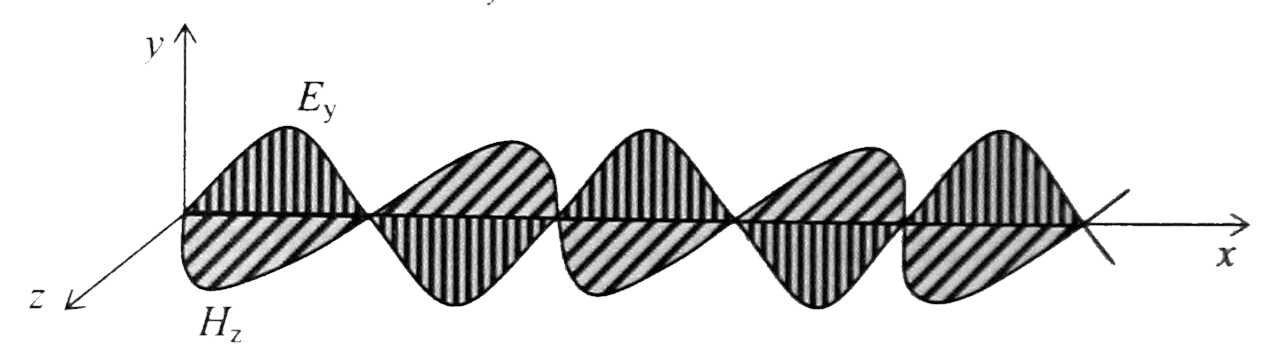
\includegraphics[width=0.9\linewidth]{patocka_elmgp03.png}
          \caption{Průběhy složek \(E_y\) a \(H_z\) v rovinné vlně, orientované paralelně s rovinou 
                   \(y-z\). Vlna se šíří vakuem nebo izolantem ve směru kladné osy \(x\). Její 
                   amplitudy jsou konstantní netlumené. \cite[s.~77]{Patocka4}.}
          \label{ES:fig_elmgp03}
        \end{figure}
        
      \subsubsection{Poyntinguv vektor}
        \begin{align}\label{ES:eq_elmagp41}
          \Gamma_\text{č} \equiv \Gamma_\text{stř}
            &= \frac{1}{2}\Re\left[\hat{E}\hat{H}^*\right]      
             = \frac{1}{2}EH                                            \nonumber\\
            &= \frac{1}{2}\frac{E^2}{\abs{Z_0}}
            = \frac{1}{2}H^2\abs{Z_0}.
        \end{align}
        Fakt, že vlnová impedance vakua je čistě \emph{reálná}, je nutno interpretovat tak, že   
        transport energie z vysílací antény do vakua je bezeztrátový (!), tj., že vakuum je schopno 
        veškerou energii z antény přijmout. Fakt, že hloubka vniku je \emph{nekonečná}, je nutno 
        interpretovat tak, že energie se může bez útlumu šířit vakuem na libovolné vzdálenosti.

        Podobné závěry platí i pro šíření elektromagnetické vlny v \emph{izolantech}, např. v 
        plynech, sklu, vodě. Jediný rozdíl spočívá v tom, že izolanty nejsou dokonalé. Mají konečně 
        velký měrný odpor \(\varrho\), proto dochází k většímu či menšímu exponenciálnímu útlumu 
        vlny při jejím postupu, viz následující kapitolu.

    \subsection{Rovinná vlna v prostředí s malou vodivostí nebo při vysokých kmitočtech}
      U vodičů, polovodičů a izolantů lze definovat tzv. \textbf{relaxační dobu}:
      \begin{equation}\label{ES:eq_elmagp42}
        \tau = \varrho\varepsilon
      \end{equation}
      Relaxační doby jsou pro vodivé látky velmi malé, pro kovy řádově \SI{10e-7}{\s}. Tomu 
      odpovídá čas potřebný k rovnoměrnému rozprostření náboje na povrchu vodiče v úlohách 
      elektrostatiky. Měření relaxační doby kovů je velmi obtížné s ohledem na její nepatrnou 
      délku. Z údajů je možné nepřímo určit permitivitu elektricky vodivých kovů\footnote{U 
      kovů není jiná metoda měření permitivity možná s ohledem na jejich velkou vodivost.}, která 
      činí řádově \(\varepsilon_r \approx 100\). Relaxační doby dobrých izolantů jsou mnohem delší, 
      např. porcelán dosahuje asi \SI{100}{\s}. Tato kapitola se týká případů, kdy platí nerovnost
      \begin{equation}\label{ES:eq_elmagp43}
        \omega\varrho\varepsilon > 1.
      \end{equation}
      Pak lze obecné vztahy (\ref{ES:eq_elmagp16a}), (\ref{ES:eq_elmagp16a}) přibližně zjednodušit 
      do následující podoby.

    \subsubsection{Fázová konstanta \(\alpha\), činitel tlumení \(\beta\), hloubka vniku 
                     \(\delta\)}
       \begin{equation}\label{ES:eq_elmagp44}
         \alpha \cong \omega\sqrt{\mu\varepsilon}, \qquad
         \beta  \cong \frac{1}{2\varrho}\sqrt{\frac{\mu}{\varepsilon}}, \qquad
         \delta = \frac{1}{\beta}\cong2\varrho\sqrt{\frac{\varepsilon}{\mu}}
       \end{equation}

    \subsubsection{Fázová rychlost}
    \begin{equation}\label{ES:eq_elmagp45}
      v \cong \frac{1}{\sqrt{\mu\varepsilon}}.
    \end{equation}
    
    \subsubsection{Vlnová impedance}
    \begin{subequations}
      \begin{align}
           Z &= \frac{E}{H} = \frac{\omega\mu}{k} 
              = \sqrt{\frac{\mu}{\varepsilon}}                             
                     \frac{1}{\sqrt{1 - j\dfrac{1}{\omega\varrho\varepsilon}}}    \nonumber \\
             &= \sqrt{\frac{\mu}{\varepsilon}}           
                     \frac{1}{\sqrt{1 + 
                        \dfrac{1}{\omega^2\varrho^2\varepsilon^2}}}e^{j\Phi} 
              = \abs{Z}e^{j\Phi}                                   \label{ES:eq_elmagp46a}  \\
        \Phi &\cong \arctan\frac{1}{2\omega\varrho\varepsilon}.    \label{ES:eq_elmagp46b}
    \end{align}
    \end{subequations}

    \subsection{Rovinná vlna ve vodivém prostředí}
      Jedná se o technicky velmi významný případ šíření elektromagnetické vlny v kovech. Zde má 
      veliký význam \emph{hloubka vniku}, která je užitečná při popisu následujících jevů:
      \begin{itemize}[noitemsep]
        \item Stínící účinek kovů v radiotechnice a při průmyslovém rušení.
        \item (Téměř dokonalý) odraz vlny od kovových ploch v radiotechnice.
        \item Magnetický skinefekt v ocelovém plechu a s ním související vířivé ztráty v železe 
              transformátorů a elektrických strojů.
        \item Elektrický skinefekt ve všech kovových vodičích v radiotechnice, ale především ve 
              vinutí výkonových impulsních transformátorů, tlumivek a elektrických strojů.
     \end{itemize}
     Tato kapitola se týká případů, kdy platí nerovnost
     \begin{equation}\label{ES:eq_elmagp46}
       \omega\varrho\varepsilon \ll 1.
     \end{equation}
     S ohledem na velmi malý odpor kovů i polovodičů je nerovnost dobře splněna i pro velmi 
     vysoké kmitočty až do oblasti \SI{100}{\GHz} (milimetrové vlny). Vlivem nerovnosti 
     (\ref{ES:eq_elmagp46}) lze obecný výraz (\ref{ES:eq_elmagp15}) pro činitel šíření \(k\) 
     zjednodušit následujícím způsobem.
     
     \subsubsection{Činitel šíření \(k\)} 
       \begin{align}\label{ES:eq_elmagp47}
         k_{1,2} = \pm\sqrt{j\frac{\omega\mu}{\varrho}}            
                &= \pm(j-1)\sqrt{\frac{\omega\mu}{2\varrho}}      \nonumber \\
                &= \mp(1-j)\sqrt{\frac{\omega\mu}{2\varrho}} 
                 = \mp(\alpha - j\beta).
       \end{align}       

      \subsubsection{Fázová konstanta \(\alpha\), činitel tlumení \(\beta\), hloubka vniku  
                     \(\delta\)}
        \begin{equation}\label{ES:eq_elmagp48}
          \alpha = \sqrt{\frac{\omega\mu}{2\varrho}}, \qquad
           \beta = \frac{1}{\delta} = \sqrt{\frac{\omega\mu}{2\varrho}}, \qquad
          \delta = \sqrt{\frac{2\varrho}{\omega\mu}}  
        \end{equation} 
        Hloubka vniku \(\delta\) je převrácenou hodnotou činitele tlumení \(\beta\). Má význam 
        vzdálenosti, na které klesne amplituda dopředně vlny na hodnotu \(1/e\). Kladný činitel 
        šíření \(k_1 = +(\alpha - j\beta)\) odpovídá dopředně vlně postupující ve směru \(+x\), 
        záporný činitel šíření \(k_2 = -(\alpha - j\beta)\) odpovídá zpětné vlně postupující ve 
        směru \(-x\). Výsledné řešení může být v obecném případě superpozicí obou vln. V úvahu 
        připadají následující možnosti. S využitím (\ref{ES:eq_elmagp15}) lze psát:
        \begin{subequations}
          \begin{align}
            \shortintertext{vlna dopředná}
            \hat{E}_y(x,t) 
              &= E_+e^{j(\omega t - kx)}                                                \nonumber \\
              &= E_+e^{-\beta x}e^{j(\omega t - \alpha x)}         
               = E_+e^{-\frac{x}{\delta}}e^{j(\omega t-\frac{x}{\delta})} \label{ES:eq_elmagp49a} \\
            \shortintertext{vlna zpětná}
            \hat{E}_y(x,t) 
              &= E_-e^{j(\omega t - kx)}                                                \nonumber \\
              &= E_-e^{+\beta x}e^{j(\omega t+\alpha x)}    
               = E_-e^{+\frac{x}{\delta}}e^{j(\omega t+\frac{x}{\delta})} \label{ES:eq_elmagp49b} \\
            \shortintertext{vlna zpětná \(\pm\) zpětná}
            \hat{E}_y(x,t) 
              &= E_+e^{j(\omega t - kx)} \pm E_-e^{j(\omega t + kx)}                    \nonumber \\
              &= E_+e^{-\beta x}e^{j(\omega t - \alpha x)} \pm
                 E_-e^{+\beta x}e^{j(\omega t + \alpha x)}                              \nonumber \\
              &= E_+e^{-\frac{x}{\delta}}e^{j(\omega t - \frac{x}{\delta})}  \pm
                 E_-e^{+\frac{x}{\delta}}e^{j(\omega t + \frac{x}{\delta})}  \label{ES:eq_elmagp49c}
          \end{align}
        \end{subequations}
        V obecném případě nemusí mít amplitudy \(E_+\) a \(E_-\) stejnou velikost. Při analýze 
        \emph{skinefektu uvnitř tenkého plechu} lze díky osové symetrii ve směru tloušťky plechu, 
        tj. ve směru osy \(x\), položit \(E_+ = E_- = \frac{E(0)}{2}\), kde \(E(0)\) je středová 
        hodnota pro \(x = 0\). Pak je možno rovnici (3.2.4-6c) formálně upravit buď do tvaru
        \begin{subequations}
          \begin{align}
            \shortintertext{vlna dopředná + zpětná}
            \hat{E}_y(x,t) 
              &= E_+e^{j(\omega t - kx)} + E_-e^{j(\omega t + kx)}           \nonumber \\
              &= \frac{E(0)}{2}e^{j(\omega t - kx)} +  
                 \frac{E(0)}{2}e^{j(\omega t + kx)}                          \nonumber \\
              &= E(0)\cosh(jkx)e^{j\omega t}                                 \nonumber \\
              &= E(0)\cosh(1+j)\frac{x}{\delta}e^{j\omega t}   \label{ES:eq_elmagp50a} \\
            \shortintertext{nebo do tvaru:}
            \shortintertext{vlna dopředná - zpětná}
            \hat{E}_y(x,t) 
              &= E_+e^{j(\omega t - kx)} + E_-e^{j(\omega t + kx)}           \nonumber \\
              &= \frac{E(0)}{2}e^{j(\omega t - kx)} + 
                 \frac{E(0)}{2}e^{j(\omega t + kx)}                          \nonumber \\
              &= E(0)\sinh(jkx)e^{j\omega t}                                 \nonumber \\
              &= E(0)\sinh(1+j)\frac{x}{\delta}e^{j\omega t}  \label{ES:eq_elmagp50b}   
          \end{align}
        \end{subequations}
        Při analýze \emph{elektrického} i \emph{magnetického} skinefektu v tenkém plechu musí být i 
        ostatní složky \(H\), \(B\), \(J\) vnitřního pole popsány jednou z rovnic (3.2.4-6d) nebo 
        (3.2.4-6e), podle toho, zda je složka osově souměrná (sudá funkce) nebo středově souměrná 
        (lichá funkce), viz  obr. \ref{ES:fig_elmgp04}.
        \begin{figure}[ht!]
          \centering  
          \subcaptionbox{\label{es:fig_patocka_elmgp04a}}{\luafigure[0.45]{patocka_elmgp04a.png}}
          \subcaptionbox{\label{es:fig_patocka_elmgp04b}}{\luafigure[0.45]{patocka_elmgp04b.png}}
          \caption{Skinefekt v tenkém fóliovém vodiči, a) Elektrický skinefekt. Směr složek 
            \(B_y\), \(H_y\) odpovídá  PPR vůči pracovnímu proudu i(t). b) Magnetický 
            skinefekt. Směr složek \(E_y\), \(J_y\)  odpovídá v důsledku Lenzova principu 
            PLR vůči pracovnímu toku \(\Phi(t)\). \cite[s.~79]{Patocka4}.}
          \label{ES:fig_elmgp04}
        \end{figure}
        
        V obou případech na obr. \ref{ES:fig_elmgp04} teče celkový proud \(i(t)\), připadne celkový 
        magnetický tok \(\Phi(t)\), vždy ve směru \emph{podélné} osy \(z\). Přesto je rozloženi 
        elektromagnetického pole uvnitř plechu takové, jako by se jím šířily dvě rovinné 
        elektromagnetické vlny ve směru \emph{příčné} osy \(x\): přímá vlna ve směru \(+x\), 
        odražená ve směru \(-x\). Z obrázku je zřejmé, které ze složek vyhovují liché funkci typu 
        \(
        \sinh(x)\), a které sudé funkci typu \(\cosh(x)\). Typ funkce je dán konkrétními okrajovými 
        podmínkami, které budou upřesněny v příslušných kapitolách o skinefektu.
       
        \subsubsection{Fázová rychlost}
          \begin{equation}\label{ES:eq_elmagp51}
            v = \der{x}{t} = \frac{\omega}{\alpha} 
              = \sqrt{\dfrac{2\omega\varrho}{\mu}}.
          \end{equation}
          Rychlost šíření vlny v kovech je velmi závislá na kmitočtu. Je-li prostředí hodně 
          vodivé - a to platí pro všechny kovy - rychlost šíření je \emph{velmi malá}. Do vnitřního 
          prostoru supravodičů nemohou elektromagnetické vlny vůbec vniknout, protože pro \(\varrho 
          = 0\) je \(v = 0\). Povrch supravodiče se tedy chová jako \emph{dokonalé zrcadlo}. To 
          platí přibližně i pro většinu kovů, viz např. vnitřní odrazové stěny vlnovodů a 
          dutinových rezonátorů, které jsou prakticky bezeztrátové i na vysokých kmitočtech v 
          oblasti \SI{10}{\GHz} (centimetrové vlny), nebo optická zrcadla ve viditelném oboru.

        \subsubsection{Vlnová impedance prostředí}
          \begin{subequations}
            \begin{align}
                Z &= \frac{E}{H} = \frac{\omega\mu}{k} 
                   = \frac{\omega\mu}{\alpha} 
                   = (1+j)\sqrt{\frac{\mu\varrho\varepsilon}{2}}                      \nonumber \\
                  &= (1+j)\sqrt{\mu\varrho\varepsilon}\,e^{j\SI{45}{\degree}}         
                   =  \abs{Z}e^{j\SI{45}{\degree}}                      \label{ES:eq_elmagp51a} \\
             \Phi &= \arctan\frac{1}{1} 
                   = \arctan(1) 
                   = \SI{45}{\degree}                                   \label{ES:eq_elmagp51b} 
            \end{align}
          \end{subequations}
          Fázový posuv \(\Phi\) mezi oběma vektory je v kovech vždy \SI{45}{\degree}, bez ohledu na 
          velikost \(\mu\) ,\(\varrho\).
          
          \begin{figure}[ht!]
            \centering
            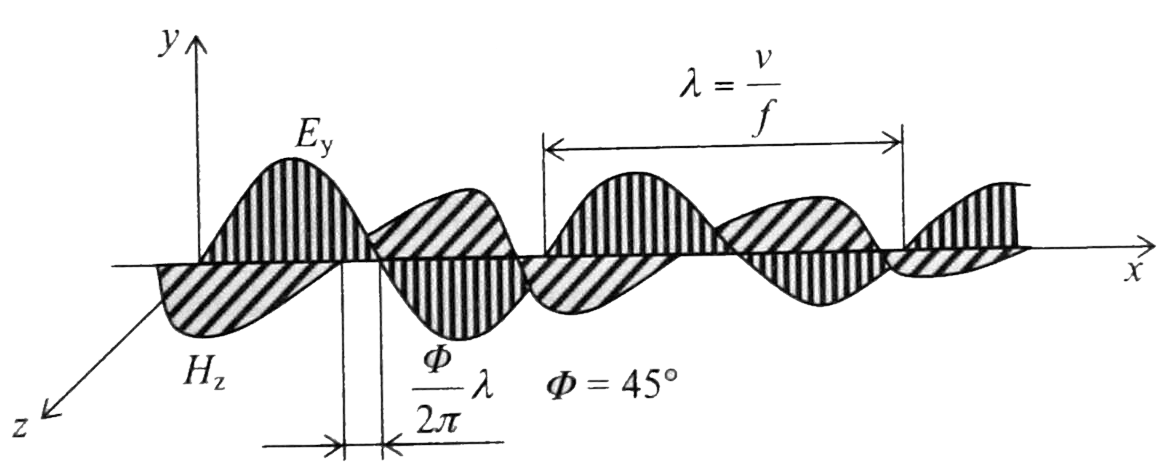
\includegraphics[width=0.85\linewidth]{patocka_elmgp05.png}
            \caption{Průběhy složek \(E_y\) a \(H_z\) v rovinné vlně, orientované paralelně s 
                     rovinou \(y-z\). Vlna se šíří kovem ve směru osy \(+x\). Tato vlna odpovídá 
                     dopředně vlně na obr. \ref{es:fig_patocka_elmgp04b}. \cite[s.~80]{Patocka4}.}
            \label{ES:fig_elmgp05}
          \end{figure}
                
        \subsubsection{Poyntingův vektor}
          \begin{align}\
            \Gamma_\text{č} \equiv \Gamma_\text{stř} 
              &= \frac{1}{2}\Re\left[\hat{E}\hat{H}^*\right] 
               = \frac{1}{2}\Re\left[\hat{E}^*\hat{H}\right]     
               = \frac{1}{2}EH\cos(\SI{45}{\degree})                 \nonumber \\ 
              &= \frac{1}{2}EH\frac{1}{\sqrt{2}}
               = \frac{1}{2\sqrt{2}}\frac{E^2}{\abs{Z}}
               = \frac{1}{2\sqrt{2}}H^2\abs{Z}.                      \label{ES:eq_elmagp52}
          \end{align}
%~~~~~~~~~~~~~~~~~~~~~~~~~~~~~~~~~~~~~~~~~~~~~~~~~~~~~~~~~~~~~~~~~~~~~~~~~~~~~~~~~~~~~~~~~~~~~~~~~~